\documentclass[preprint,12pt]{elsarticle}

\usepackage{amsmath}
\usepackage{amssymb}
\usepackage{graphicx}
\usepackage{booktabs}
\usepackage[hidelinks]{hyperref}

\graphicspath{{../../services/inference/data/final/report/}{../../services/inference/data/figures/}}

\journal{Physica A}

\begin{document}

\begin{frontmatter}

\title{A cortical-proxy observable for emotionally manipulative media: an instrument, a
400-item corpus, and the field bound it yields}

\author[cuea]{Brian Mwai}
\ead{mwaibryn@gmail.com}
\address[cuea]{Department of Natural Sciences, Faculty of Science, The Catholic University of
Eastern Africa, P.O. Box 62157-00200, Nairobi, Kenya}

\begin{abstract}
Mean-field opinion models treat media as an external field on a population of coupled
states, and that field is almost never measured. A companion paper \cite{mwai_bound} states what any candidate
observable must satisfy for the mechanism to operate: $\alpha \ge h_c(\beta J)/\Delta X$.
This paper supplies the missing half, an observable computed from content and the spread it
attains on a real corpus. Text is spoken, transcribed, embedded and passed to a released
trimodal encoder that predicts cortical response; two networks are averaged from that
prediction, one associated with affective salience and one with deliberative control, and the
observable is their signed difference. The ratio form is undefined for $17.25\%$ of items and
is replaced by that difference. On 400 items across four categories, matched on length, the
categories separate at $\eta^2 = 0.1068$, $F = 15.779$, $p = 1.035\times10^{-9}$, against a
design powered to detect $\eta^2 = 0.0268$. The separation is carried by fear-activating
content, $d = 0.9389$ against neutral, while high-outrage content does not separate,
$d = 0.0300$, because it raises both networks by nearly equal amounts. Each category is drawn
from one source dataset, so the separation is between corpora and cannot be attributed to
framing; we state this before the result rather than in limitations. Against the pre-scan
manipulative label the observable reaches $\mathrm{AUC} = 0.6274$, and a TF-IDF baseline on
the same rows reaches $0.9758$, so the observable is offered as a field quantity and not as a
classifier. A second scanning session gives test-retest $\mathrm{ICC} = 0.8725$ and
replicates the separation at $\eta^2 = 0.0888$, while $12.8\%$ of individual items reverse
direction, a count that additive noise at the measured session error predicts, so the
instrument supports category-level statements and no per-item verdict.
Calibrating the coupling does not identify it: the fit performs worse than the sample mean
out of sample and scales with an unmeasured $\beta J$, so no value is quoted. What the
measurement does yield is the spread, $\Delta X = 0.1241$, which converts the companion
paper's inequality into a concrete requirement, $\alpha \ge 4.2938$ at $\beta J = 2$, on any
study proposing this mechanism.
\end{abstract}

\begin{keyword}
sociophysics \sep opinion dynamics \sep external field \sep media measurement \sep
encoding models \sep reproducibility
\end{keyword}

\end{frontmatter}

\section{Introduction}

Statistical-physics treatments of opinion formation routinely include a term representing
media. In the mean-field Ising formulation and its relatives \cite{castellano2009,galam2008}, that term is an external field
$h$ acting on every agent, and the modelling result is that beyond a critical magnitude
$h_c(\beta J)$ the population is driven from one consensus to another. The literature on this
mechanism is large \cite{crokidakis2012,azhari2023,freitas2020,sirbu2016} and the qualitative
conclusion is robust within the models.

The field itself is almost never measured. It is assigned, swept, or fitted to an outcome
that the model was built to reproduce. A companion paper \cite{mwai_bound} makes the consequence precise:
writing $h = \alpha X$ for a content observable $X$ with attainable range $\Delta X$, no
media-driven transition across the spinodal of the all-to-all mean-field model is possible
unless
\begin{equation}
\label{eq:bound}
\alpha \ \ge\ \frac{h_c(\beta J)}{\Delta X},
\end{equation}
and this can be evaluated before any data are collected. What it cannot supply is
$\Delta X$, which is an empirical property of a real observable on real content.

This paper supplies one. We build an instrument that computes a candidate observable from
content, apply it to a corpus assembled for the purpose, and report the spread it attains
together with what the measurement does and does not support. Three commitments run through
the work and are stated here so the reader can hold us to them: the physics stays in front
and the encoder is treated as a thermometer rather than a subject; every number is written by
a named script into an artifact and read from there rather than transcribed; and the design's
confound is stated before each result it touches, not deferred.

\section{The observable}
\label{sec:observable}

\subsection{Definition}

Let $A_{\text{aff}}$ be the mean predicted activation over a union of regions associated with
affective salience, and $A_{\text{del}}$ the corresponding mean over regions associated with
deliberative control. The proposal for this work specified a ratio,
\begin{equation}
\mathrm{NAA}_{\text{ratio}} \;=\; \frac{A_{\text{aff}}}{A_{\text{del}} + \delta},
\end{equation}
which is a magnitude asymmetry only when both means sit at or above baseline. The encoder's
outputs are standardised and unconstrained in sign, and a negative denominator makes the
ratio change sign for reasons that have nothing to do with the content. Across the corpus
reported below the ratio is undefined for 69 of 400 items, $17.25\%$. This is not an edge
case to be dropped, so the analysis is carried by the signed difference
\begin{equation}
\label{eq:naa}
X \;\equiv\; \mathrm{NAA}_{\text{signed}} \;=\; A_{\text{aff}} - A_{\text{del}},
\end{equation}
which is defined everywhere. Positive means affective activation is predicted to lead,
negative means deliberative activation leads. The reformulation changes what the index means:
it reports which system leads, not by what proportion.

\subsection{What the observable is not}

The observable is a \emph{cortical proxy}. The released checkpoint predicts activity on the
cortical surface only, so no subcortical structure is measured and none is named. No
participant was scanned at any point in this work: every value is a prediction produced by an
encoder from content, and the phrase ``predicted activation'' is used throughout in place of
any claim about measured brain activity.

\section{Instrument and corpus}

\subsection{The cascade}

Each item is converted to speech, transcribed with word-level timings, embedded as text and
as audio, and passed to TRIBE v2, a released trimodal encoder that predicts fMRI response
over $20{,}484$ fsaverage5 vertices \cite{tribe2025}. The checkpoint is loaded in the
average-subject configuration its own loader forces. Regions of interest are resolved once
into vertex index sets and cached, so every item is reduced over identical regions: 1030
vertices for the affective union and 851 for the deliberative union.

\begin{figure}[htbp]
\centering
\includegraphics[width=0.9\textwidth]{B1_roi_definition.pdf}
\caption{The two regions the observable is reduced over, on the cortical surface. The
affective-salience union covers 1030 vertices and the deliberative-control union 851. Both
are resolved once into vertex index sets and cached, so every item is averaged over identical
regions.}
\label{fig:roi}
\end{figure}

\subsection{Corpus design}

The corpus is 400 items in four categories of 100, matched on length. Mean word counts are
$167.4$, $163.5$, $163.7$ and $162.2$ for fear-activating, high-outrage, neutral and
reward-hook items respectively, with standard deviations between $10.2$ and $12.8$, so length
is not a confound.

\begin{table}[htbp]
\centering
\begin{tabular}{@{}llr@{}}
\toprule
\textbf{Category} & \textbf{Source} & \textbf{n} \\
\midrule
Fear activating       & ISOT-fake             & 100 \\
High outrage          & SemEval-2019 Task 4   & 100 \\
Reward hook           & Webis-Clickbait-17    & 100 \\
Neutral informational & PubMed, ISOT-true     & 50 + 50 \\
\bottomrule
\end{tabular}
\caption{Corpus composition. Each category is drawn from exactly one source dataset, which is
the study's dominant limitation and is stated before every result it affects. Sources:
ISOT \cite{ahmed2017}, SemEval-2019 Task~4 \cite{kiesel2019}, Webis-Clickbait-17
\cite{potthast2018}, PubMed \cite{pubmed}.}
\label{tab:corpus}
\end{table}

\textbf{The corpus is not source-balanced, and this is the central caveat of the paper.}
Category and provenance coincide by construction, so any separation the instrument reports is
a separation between corpora and cannot be attributed to framing. Section~\ref{sec:results}
states this alongside the result rather than after it, and Section~\ref{sec:whatsurvives}
identifies which conclusions survive it.

Items were scanned interleaved rather than one category at a time. This turns out to matter,
for the reason given in Section~\ref{sec:reliability}.

\section{Results}
\label{sec:results}

All values below are read from \texttt{data/final/rq\_answers.json}, written by
\texttt{scripts/analyze\_corpus.py} from the scan output, which was itself verified
row-for-row against the source corpus on text, category and identifier.

\subsection{Separation across categories}

The four categories differ at
\begin{equation}
F = 15.779, \qquad p = 1.035\times10^{-9}, \qquad \eta^2 = 0.1068,
\end{equation}
on $n = 400$. The design was fixed before the scan and can detect $\eta^2 = 0.0268$ at
$\alpha = 0.05$ and power $0.80$, so the observed effect is roughly four times the smallest
the study could have found.

\emph{Read this with Table~\ref{tab:corpus} in view.} The categories are corpora. The
measurement establishes that the instrument assigns systematically different values to four
groups of documents; it does not establish that framing is what it responds to.

\begin{table}[htbp]
\centering
\begin{tabular}{@{}lrrr@{}}
\toprule
\textbf{Category vs neutral} & \textbf{t} & \textbf{p} & \textbf{Cohen's d} \\
\midrule
Fear activating & $+6.639$ & $3.283\times 10^{-10}$ & $+0.939$ \\
Reward hook     & $+2.254$ & $2.539\times 10^{-2}$  & $+0.319$ \\
High outrage    & $+0.212$ & $8.320\times 10^{-1}$  & $+0.030$ \\
\bottomrule
\end{tabular}
\caption{Welch comparisons against neutral informational content. The separation is carried
by fear-activating items. High-outrage items do not separate, and that is the category the
study's hypothesis expected to separate most.}
\label{tab:welch}
\end{table}

Two features of Table~\ref{tab:welch} deserve emphasis. First, the effect is one category:
remove fear-activating items and little remains. Second, high outrage does not separate on
the observable despite being drawn from its own distinct source. Section~\ref{sec:components}
shows why, and the answer is not that outrage content leaves the encoder unmoved.

Every category mean is negative, so deliberative activation is predicted to lead throughout.
The instrument finds no affective dominance anywhere in this corpus.

\begin{figure}[htbp]
\centering
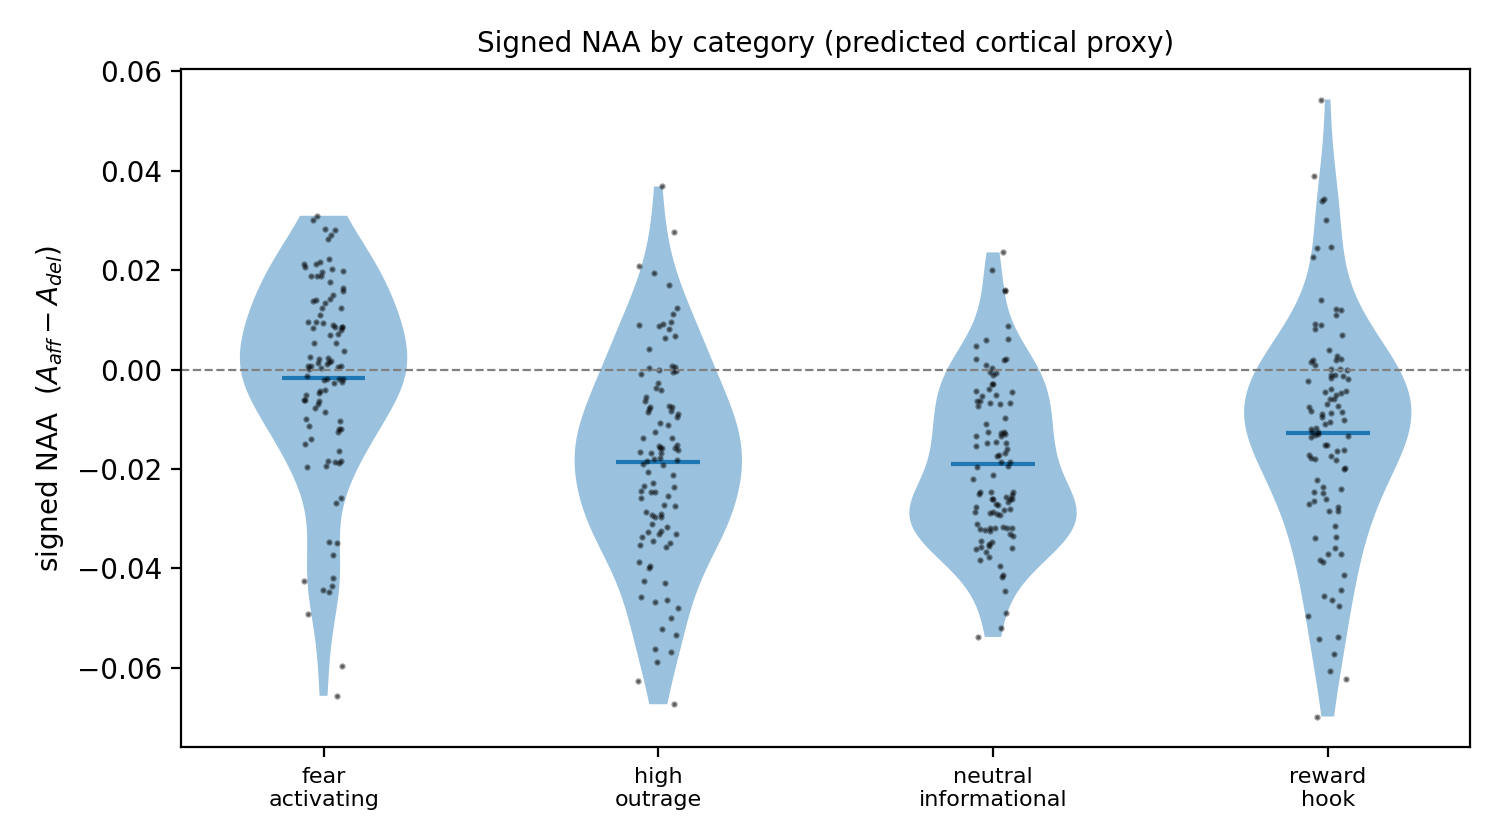
\includegraphics[width=0.9\textwidth]{fig_violin.png}
\caption{Distribution of the signed observable within each category, all 400 items. Every
category mean is negative, so deliberative activation is predicted to lead throughout, and
the separation is a shift between overlapping distributions rather than a clean split.}
\label{fig:violin}
\end{figure}

\subsection{The two components, taken separately}
\label{sec:components}

The observable is a difference, and a difference cannot tell a large symmetric response from
no response. Both components are recorded per item, so each can be compared against neutral
content on its own.

\begin{table}[htbp]
\centering
\begin{tabular}{@{}llrrr@{}}
\toprule
\textbf{Category vs neutral} & \textbf{Component} & \textbf{t} & \textbf{p} & \textbf{Cohen's d} \\
\midrule
Fear activating & $A_{\text{aff}}$ & $+4.333$ & $2.365\times 10^{-5}$  & $+0.613$ \\
Fear activating & $A_{\text{del}}$ & $-0.696$ & $4.875\times 10^{-1}$  & $-0.098$ \\
\midrule
High outrage    & $A_{\text{aff}}$ & $+3.584$ & $4.263\times 10^{-4}$  & $+0.507$ \\
High outrage    & $A_{\text{del}}$ & $+3.468$ & $6.521\times 10^{-4}$  & $+0.491$ \\
\midrule
Reward hook     & $A_{\text{aff}}$ & $+1.842$ & $6.691\times 10^{-2}$  & $+0.261$ \\
Reward hook     & $A_{\text{del}}$ & $-0.063$ & $9.501\times 10^{-1}$  & $-0.009$ \\
\bottomrule
\end{tabular}
\caption{Welch comparisons of each component against neutral informational content. High
outrage moves both components by nearly the same amount; fear-activating content moves one.}
\label{tab:component-welch}
\end{table}

High outrage raises $A_{\text{aff}}$ by $d = +0.507$ and $A_{\text{del}}$ by $d = +0.491$, both
at $p < 10^{-3}$, and the difference between them by $d = +0.030$. The category that fails to
separate on the observable is the one that moves both networks together. Fear-activating
content raises $A_{\text{aff}}$ by $d = +0.613$ and leaves $A_{\text{del}}$ flat, so its whole
effect on the observable is one-sided. A one-way ANOVA on each component alone gives
$F = 7.451$ for $A_{\text{aff}}$ and $F = 6.399$ for $A_{\text{del}}$, both $p < 10^{-3}$.

This weakens an argument we would otherwise make. If outrage had moved neither component, its
failure to separate would count against the instrument simply detecting provenance. It moves
both, so every category drawn from a distinct source does move away from the baseline on at
least one component, which is what source detection predicts. The components do not resolve
the confound in either direction.

\begin{figure}[htbp]
\centering
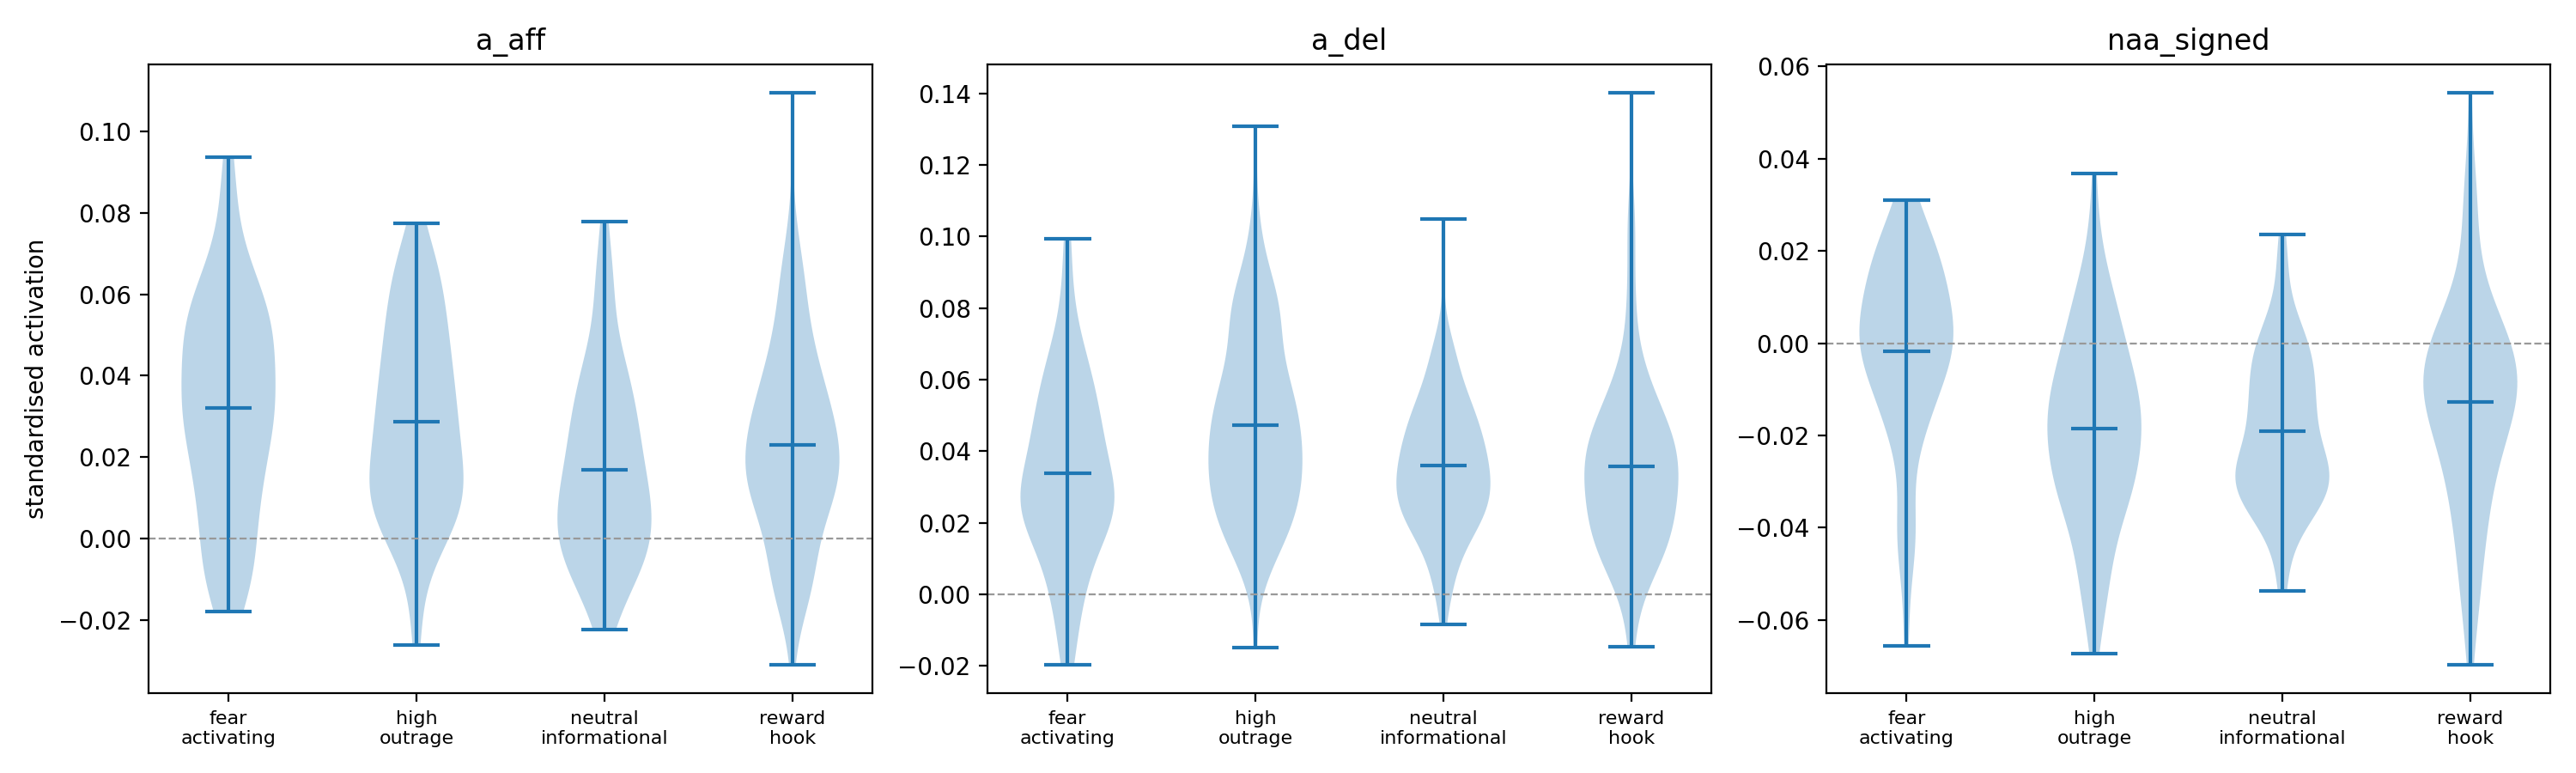
\includegraphics[width=0.95\textwidth]{fig_components.png}
\caption{$A_{\text{aff}}$, $A_{\text{del}}$ and their signed difference by category over all
400 items. High outrage is elevated on both components and flat on the difference.}
\label{fig:components}
\end{figure}

\subsection{Discrimination against the pre-scan label}

Against the \texttt{manipulative} label carried by each item before it was scanned, the
observable discriminates at $\mathrm{AUC} = 0.6274$, above the smallest detectable
$0.5916$. AUC is the headline because it is threshold-free. An $F_1$ of $0.6680$ is
obtainable, but its threshold was chosen on the same data it is evaluated on, and it is
labelled as fitted in sample wherever it appears.

An AUC has no meaning without a baseline, so two were run on the same rows and label by
\texttt{scripts/baselines.py}: TF-IDF over unigrams and bigrams with logistic regression,
scored out of fold under five-fold stratified cross-validation, and the VADER \cite{hutto2014} compound
sentiment score used directly with nothing fitted. Intervals are $2{,}000$-draw bootstrap
percentiles.

\begin{table}[htbp]
\centering
\begin{tabular}{@{}llrrl@{}}
\toprule
\textbf{Model} & \textbf{Split} & \textbf{n} & \textbf{AUC} & \textbf{95\% CI} \\
\midrule
Observable $X$     & nothing fitted    & 400 & $0.6274$ & $[0.5702, 0.6867]$ \\
VADER compound     & nothing fitted    & 400 & $0.5392$ & $[0.4757, 0.6035]$ \\
TF-IDF + logistic  & 5-fold stratified & 400 & $0.9758$ & $[0.9601, 0.9879]$ \\
\midrule
Observable $X$     & ISOT only         & 150 & $0.7290$ & $[0.6431, 0.8132]$ \\
VADER compound     & ISOT only         & 150 & $0.4019$ & $[0.3098, 0.4943]$ \\
TF-IDF + logistic  & ISOT only, 5-fold & 150 & $0.9724$ & $[0.9483, 0.9901]$ \\
\bottomrule
\end{tabular}
\caption{Baselines against the same label. The lower block keeps only the 150 items from the
ISOT collection, the one origin corpus contributing both classes.}
\label{tab:baselines}
\end{table}

\textbf{The lexical baseline wins by a wide margin.} Sentiment does not clear chance. The
observable is not a better detector of manipulative content than counting words, and no such
claim is made. Leave-one-source-out, the natural correction for the confound, is unavailable
because every source contributes exactly one class, so a held-out source leaves a single-class
test fold. The ISOT-only block is the substitute, and TF-IDF holds at $0.9724$ there. Both
TF-IDF figures nonetheless sit above $0.95$, where near-ceiling lexical performance on a small
split points to residual stylistic markers, and a probe on the same features recovers the
source dataset at $66.25\%$ against $25\%$ chance. Much of what the lexical model separates is
provenance. The observable is carried forward as the field quantity Eq.~\eqref{eq:bound}
consumes, not as a competing classifier.

\begin{figure}[htbp]
\centering
\includegraphics[width=0.95\textwidth]{B3_per_vertex_fear_activating-0000.pdf}
\caption{Predicted response for one fear-activating item at every one of the 20{,}484
cortical vertices, on the pial surface. Vertices below the map's 70th percentile are left
unpainted so the anatomy remains readable, and the threshold is stated in the figure. This is
the encoder's own output, not a smoothed or interpolated field.}
\label{fig:pervertex}
\end{figure}

\subsection{Session reliability}
\label{sec:reliability}

A second GPU session rescanned all 400 items with identical text, identical code and
identical region definitions. That pair is a test-retest measurement, and without it every
effect above would rest on a single session with no statement of how much of an item's score
is the item and how much is the session.

\begin{table}[htbp]
\centering
\begin{tabular}{@{}lrrrr@{}}
\toprule
& $r$ & ICC(2,1) & $\mathrm{sd}(\Delta)$ & $\mathrm{sd}(\Delta)/\mathrm{sd}_{\text{between}}$ \\
\midrule
$\mathrm{NAA}_{\text{signed}}$ & $0.8763$ & $0.8725$ & $0.01029$ & $0.484$ \\
$A_{\text{aff}}$ & $0.8759$ & $0.8713$ & $0.01213$ & $0.489$ \\
$A_{\text{del}}$ & $0.8576$ & $0.8550$ & $0.01271$ & $0.521$ \\
\bottomrule
\end{tabular}
\caption{Agreement between two scanning sessions over all 400 items. ICC is
reported beside $r$ because a session that shifted every score by a constant would still
correlate perfectly.}
\label{tab:retest}
\end{table}

Three consequences follow, and they cut in different directions.

\textbf{The separation replicates.} On the second session the four-category ANOVA gives
$\eta^2 = 0.0888$, $F = 12.861$, $p = 4.918\times10^{-8}$, against $\eta^2 = 0.1068$,
$F = 15.779$ for the first session over the same items. Both clear the detectable
floor. The result is not an artifact of one session. The second session's effect is roughly
a fifth smaller; both sessions carry the same error, so the difference is within what sampling
variation between two noisy runs produces.

\textbf{Per-item direction is not reliable.} Of 400 paired items, 51, or $12.8\%$, reverse
sign between sessions. A statement that a particular item is affective-leading is therefore
not supportable at this precision, and no per-item verdict appears anywhere in this paper or
in the public interface described in Section~\ref{sec:availability}. Group means over 100
items average this scatter down by an order of magnitude, which is why the category-level
result survives.

\textbf{The reversal count is the measured noise, not an extra defect.} The paired differences
give a per-session error $\sigma = \mathrm{sd}(\Delta)/\sqrt{2} = 0.00728$, against a
between-item standard deviation of $0.01913$ once that error is removed. Under additive error
at that $\sigma$, with each item's value shrunk toward the grand mean so that no item's own
noise predicts its own reversal, $20{,}000$ simulations give $55.3$ expected reversals, $95\%$
interval $[44, 67]$. The observed $51$ sits inside it. Reversing items sit near zero, mean
$|X| = 0.00320$ against $0.02159$ ($p = 1.4\times10^{-25}$), and spread evenly across
categories ($\chi^2 = 2.764$, $p = 0.429$). Per-item direction is therefore out of reach at
this $\sigma$, rather than awaiting a fix.

\textbf{Scan order does not carry the separation.} Because the corpus took more than one
session, position in the scan is a candidate explanation for the category effect. It is not
one. Items were scanned interleaved, so the four categories are balanced across thirds of the
scan order, $\chi^2 = 3.139$, $p = 0.7913$. The drift is real, $\eta^2 = 0.0167$ at
$p = 0.0353$, but it is orthogonal to category by construction: removing scan-third means
before the category ANOVA moves the effect only from $\eta^2 = 0.1068$ to $0.1048$,
$p = 1.588\times10^{-9}$. Had the corpus been scanned one category at a time, this drift
would have been indistinguishable from the finding.

Neither session is corrected toward the other and the two are not averaged. An average of two
sessions would carry a precision that neither run has.

\section{The physics}

\subsection{Calibration does not identify the coupling}

With the observable in hand, the natural step is to estimate $\alpha$ in $h = \alpha X$ by
fitting the model's predicted outcome against the corpus. On partial runs the bootstrap
interval for $\hat{\alpha}$ comfortably included zero. On the completed corpus it no longer
does. That is not a result, for two reasons.

The fit performs worse than the sample mean on held-out data, so it has no out-of-sample
predictive value: a negative held-out $R^2$ means the relationship it encodes does not
generalise beyond the points used to estimate it. And the estimate scales inversely with
$\beta J$, which nothing in this study measures, so any single value reported would be a
statement about a chosen $\beta J$ rather than about media.

The coupling is therefore \emph{unidentified}, which is a weaker claim than either a
detection or a null. \textbf{No value of $\hat{\alpha}$ is quoted in this paper}, in text,
table or caption.

\begin{figure}[htbp]
\centering
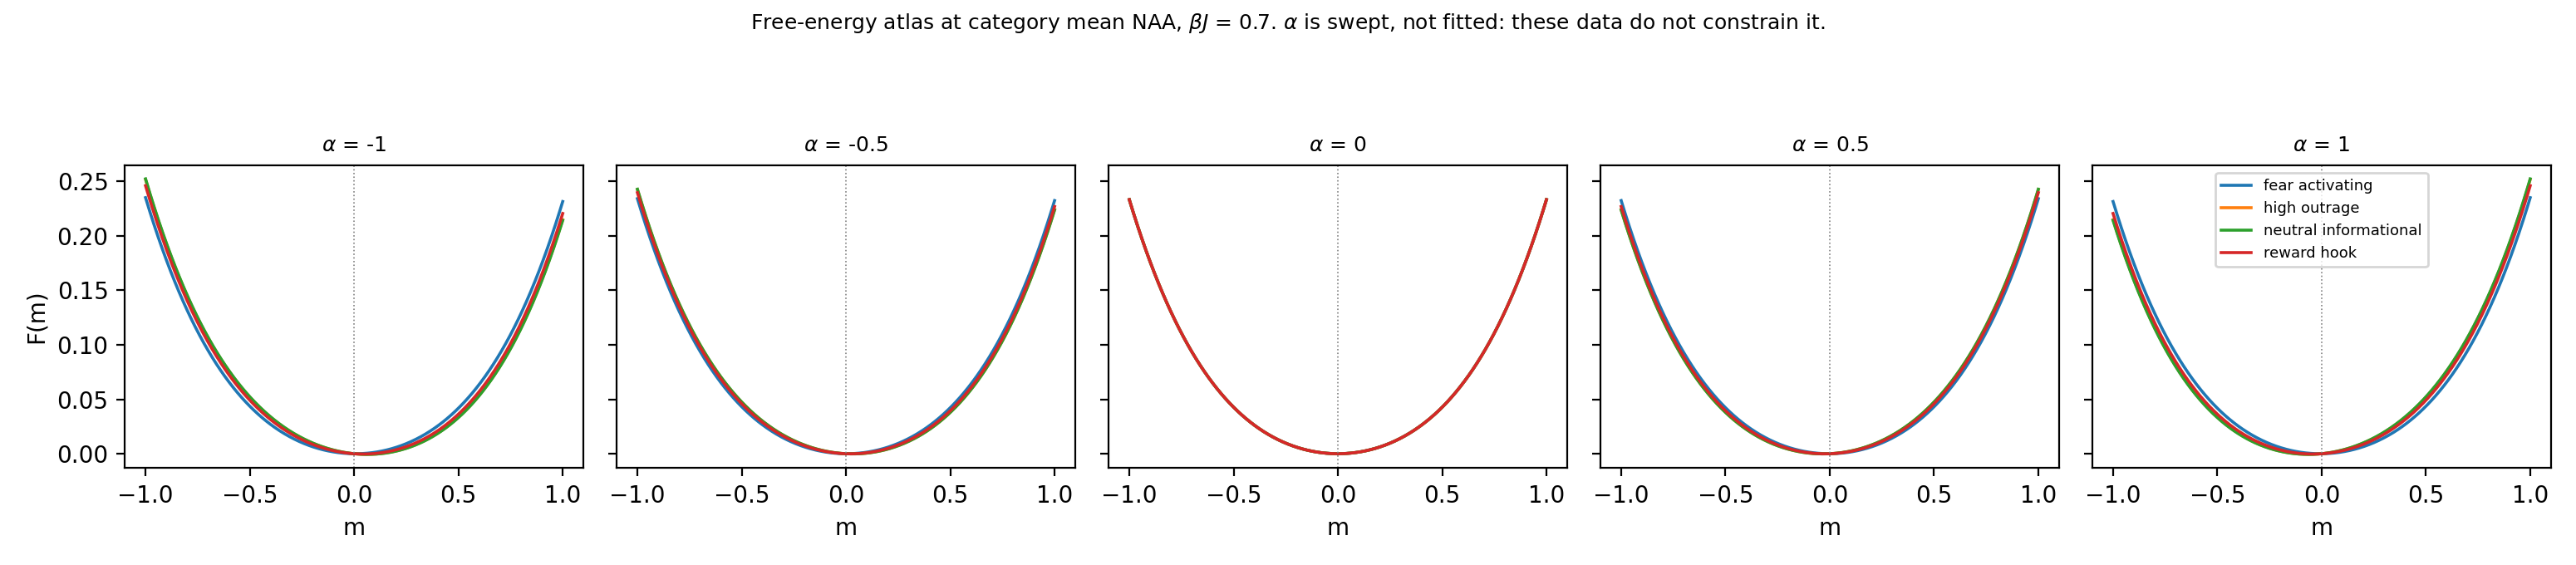
\includegraphics[width=0.9\textwidth]{fig_free_energy_atlas.png}
\caption{Free energy swept across a range of couplings, evaluated at each category's measured
mean. The sweep is not a fit: no value of $\alpha$ is estimated from the data anywhere in
this paper, and the panels show how the physics would behave for each coupling rather than
which coupling holds.}
\label{fig:freeenergy}
\end{figure}

\subsection{What the spread does yield}

The measurement does deliver the quantity Eq.~\eqref{eq:bound} consumes. Across the corpus
the observable attains
\begin{equation}
\Delta X = 0.1241,
\end{equation}
and substituting into the companion paper's inequality converts a general statement into a
concrete requirement.

\begin{table}[htbp]
\centering
\begin{tabular}{@{}lrr@{}}
\toprule
$\beta J$ & $h_c(\beta J)$ & $\alpha$ required \\
\midrule
$1.102$ & $0.02101$ & $0.1693$ \\
$1.496$ & $0.20541$ & $1.6553$ \\
$2.000$ & $0.53284$ & $4.2938$ \\
\bottomrule
\end{tabular}
\caption{The field bound evaluated at three reduced couplings, using the measured spread
$\Delta X = 0.1241$. Each row states the coupling any proposal of this mechanism would need
in order for media to drive a transition through this observable.}
\label{tab:bound}
\end{table}

This is a necessary condition and not a sufficient one. Clearing it does not establish that
media moves populations; falling below it excludes the mechanism within the model.

\section{What survives the confound}
\label{sec:whatsurvives}

It is worth separating the claims this study can defend from those it cannot, because the two
are easy to conflate.

\emph{Not supported.} That the instrument detects manipulation, or does so better than a
lexical model. That framing rather than provenance drives the separation. Any value for the coupling. Any statement about an
individual item. Any claim about subcortical structures, or about measured rather than
predicted activity.

\emph{Supported.} That the observable attains a measured spread of $0.1241$ on real content,
which is what the bound consumes and which does not depend on why the spread arises. That the
categories separate at an effect four times the detectable floor, and that the separation
replicates in an independent session. That high-outrage content, the category the
hypothesis favoured most, raises both networks together and so leaves the observable where
neutral content puts it. And that the coupling is unidentified on this data, which constrains what a
successor may assume.

The confound is removable by design rather than by analysis. Drawing all four categories from
a single source, so that provenance is held constant while framing varies, or crossing
sources with categories so that the two are statistically separable, would convert the
present result into an interpretable one. Neither requires new instrumentation.

\section{Limitations}

\begin{enumerate}
\item Category is confounded with source dataset. The dominant limitation, stated in
Section~\ref{sec:results} as well as here.
\item Single-session scores are noisy: $\mathrm{ICC} = 0.8725$, with session-to-session
standard deviation $48.4\%$ of the between-item standard deviation. Category-level
conclusions survive this; per-item ones do not.
\item Predicted activation is not measured activation. Whether the encoder tracks real cortex
is unresolved and contested; a published audit reports the released average-subject
checkpoint anti-correlated with cortex \cite{sapient2026}, and a parcel-level replication on
public data \cite{mwai_encoder} does not find that sign but is not yet decisive.
\item Cortical proxy only. The checkpoint cannot speak to subcortical structure.
\item Average-subject configuration, forced by the loader.
\item Out-of-distribution stimuli: the encoder was trained on naturalistic audiovisual
material and is given synthesised speech from written text.
\item The corpus is English-language from five specific sources, none of them African. A
search for openly licensed African news data carrying usable labels returned nothing
suitable, so the spread is a property of American and European publishing and the bound
inherits that limitation.
\end{enumerate}

\section{Conclusion}

Media enters mean-field opinion models as a field that is almost never measured. This paper
measured a candidate: an observable computed from content through a released cortical
encoder, applied to 400 items, with its spread, its reliability and its failure modes
reported rather than assumed. The instrument separates four corpora at an effect it was
powered to find, the separation replicates across sessions, and it is confounded with
provenance in a way no analysis of this corpus can undo. The coupling it was built to
calibrate is unidentified. What survives is the spread, and through the companion paper's
inequality a requirement, $\alpha \ge 4.2938$ at $\beta J = 2$, that any future proposal of
this mechanism must meet within all-to-all mean-field theory.

\section*{Code and data availability}
\label{sec:availability}

The pipeline, corpus builder, analysis and figure scripts, and the JSON and CSV artifacts
every number above is read from, are public at \url{https://github.com/brn-mwai/monarch}. The
instrument runs at \url{https://monarch-4iy.pages.dev}, carrying the full corpus with each
item's text, its pre-scan labels and its measured values, and reporting no per-item verdict
for the reason given in Section~\ref{sec:reliability}. Figures showing predicted responses
are generated by \texttt{scripts/render\_brain\_figures.py} from the saved per-vertex maps,
each stating its threshold, rather than captured from the interface.


\section*{CRediT authorship contribution statement}

\textbf{Brian Mwai:} Conceptualization, Methodology, Software, Validation, Formal analysis,
Investigation, Data curation, Writing -- original draft, Writing -- review and editing,
Visualization. The author is the sole contributor to this work.

\section*{Declaration of competing interest}

The author declares no competing financial interests or personal relationships that could
have appeared to influence the work reported in this paper.

\section*{Funding}

This research received no specific grant from any funding agency in the public, commercial or
not-for-profit sectors. Computation was carried out on publicly available free-tier resources.

\section*{Acknowledgements}

The author thanks Dr.\ Songa Mutambi of the Department of Natural Sciences, The Catholic University of
Eastern Africa, for supervising the project of which this work forms part. The supervision was
academic guidance and approval; the author is solely responsible for the content.

\begin{thebibliography}{9}

\bibitem{tribe2025}
S.~d'Ascoli, J.~Rapin, Y.~Benchetrit, H.~Banville, J.-R.~King,
TRIBE: TRImodal Brain Encoder for whole-brain fMRI response prediction, arXiv:2507.22229
(2025).

\bibitem{castellano2009}
C.~Castellano, S.~Fortunato, V.~Loreto,
Statistical physics of social dynamics,
Rev. Mod. Phys. 81 (2009) 591--646.

\bibitem{galam2008}
S.~Galam,
Sociophysics: A review of Galam models,
Int. J. Mod. Phys. C 19 (2008) 409--440.

\bibitem{crokidakis2012}
N.~Crokidakis,
Effects of mass media on opinion spreading in the Sznajd sociophysics model,
Physica A 391 (2012) 1729.

\bibitem{azhari2023}
Azhari, R.~Muslim,
The external field effect on opinion formation based on the majority rule and the $q$-voter
models on the complete graph,
Int. J. Mod. Phys. C (2023) 2350088.

\bibitem{freitas2020}
F.~Freitas, A.~R.~Vieira, C.~Anteneodo,
Imperfect bifurcations in opinion dynamics under external fields,
J. Stat. Mech. (2020) 024002.

\bibitem{sirbu2016}
A.~S\^{i}rbu, V.~Loreto, V.~D.~P.~Servedio, F.~Tria,
Opinion dynamics: models, extensions and external effects,
in: Participatory Sensing, Opinions and Collective Awareness, Springer, 2016, pp. 363--401.

\bibitem{mwai_bound}
B.~Mwai,
Bounding the external field in mean-field opinion dynamics: what any content observable must
satisfy to drive a transition, manuscript in preparation (2026).

\bibitem{mwai_encoder}
B.~Mwai,
What does a released average-subject brain encoder actually predict? A noise ceiling, a
parcel-level replication, and three silent failures, manuscript in preparation (2026).

\bibitem{ahmed2017}
H.~Ahmed, I.~Traore, S.~Saad,
Detection of online fake news using n-gram analysis and machine learning techniques,
in: ISDDC 2017, Lecture Notes in Computer Science 10618, Springer, 2017, pp. 127--138.

\bibitem{kiesel2019}
J.~Kiesel, M.~Mestre, R.~Shukla, E.~Vincent, P.~Adineh, D.~Corney, B.~Stein, M.~Potthast,
SemEval-2019 Task 4: Hyperpartisan news detection,
in: Proceedings of the 13th International Workshop on Semantic Evaluation, 2019, pp. 829--839.

\bibitem{potthast2018}
M.~Potthast, T.~Gollub, K.~Komlossy, S.~Schuster, M.~Wiegmann, E.~P.~Garces Fernandez,
M.~Hagen, B.~Stein,
Crowdsourcing a large corpus of clickbait on Twitter,
in: Proceedings of COLING 2018, pp. 1498--1507.

\bibitem{pubmed}
National Center for Biotechnology Information, PubMed, accessed through the Entrez
Programming Utilities, \url{https://pubmed.ncbi.nlm.nih.gov}.

\bibitem{hutto2014}
C.~J.~Hutto, E.~Gilbert,
VADER: A parsimonious rule-based model for sentiment analysis of social media text,
in: Proceedings of ICWSM 2014, pp. 216--225.

\bibitem{sapient2026}
The Sapient Company, The Faceless Brain, self-published technical report, 2026,
\url{https://thesapientcompany.com/research}.

\end{thebibliography}

\end{document}
